\documentclass[thesis.tex]{subfiles}

\begin{document}
Ab-initio structure calculations of many-fermion systems such as those in nuclear and electronic structure aim to describe emergent phenomena from the constituent particles subject to the underlying microscopic Hamiltonian.  This amounts to finding the solution to the many-body Schrodinger equation.  However, a calculation of the exact solution needs to account for all possible correlations among the particles and thus scales factorially.  This motivates the need for approximations to the exact solution that account for the most important correlations.  This chapter first establishes the formalism neccesary to define the many-body problem then illustrates several successive approximations to its solution.  Because the type of fermions and the underlying Hamiltonian can be kept generic until specific systems are considered, the formalism and many-body methods can be kept generic as well.


\section{Independent-Particle Model}
The nonrelativistic A-body quantum problem begins with the Schrodinger equation,
\begin{equation}
  \Ham\Psi\left(\mathbf{r}_{1},\cdots,\mathbf{r}_{A}\right) = E\Psi\left(\mathbf{r}_{1},\cdots,\mathbf{r}_{A}\right),
\end{equation}
for the correlated wave-function $\Psi\left(\mathbf{r}_{1},\cdots,\mathbf{r}_{A}\right)$ and the corresponding energy $E$.  The Hamiltonian can be written generically as a sum of $k$-body pieces which, in principle, can contain up to $A$-body interactions,
\begin{align}
  \Ham &= \HamB{1} + \HamB{2} + \HamB{3} + \cdots \notag \\
  &= \sum^{A}_{\mathclap{i}}\HamB{1}\left(\mathbf{r}_{i}\right) + \sum^{A}_{\mathclap{i<j}}\HamB{2}\left(\mathbf{r}_{i},\mathbf{r}_{j}\right) + \sum^{A}_{\mathclap{i<j<k}}\HamB{3}\left(\mathbf{r}_{i},\mathbf{r}_{j},\mathbf{r}_{k}\right) + \cdots.
\end{align}
Regardless of the system, the one-body term contains the kinetic energy operator $\frac{-\hbar^{2}}{2m}\nabla^{2}_{i}$, while the higher-order terms result from inter-particle interactions.

An intuitive way to formulate the solution to the many-body Schrodinger equation is to express the collective wave-function in terms of independent single-particle wave-functions, or orbitals $\phi$.  In this \ittext{independent-particle model}, a selection of single-particle wave-functions, known as the single-particle basis, are constructed by solving the Schrodinger equation for a single particle in some mean-field potential, for bound systems, or no potential, for infinite systems.  Then a many-body wave-function is constructed as a product of these single-particle orbits.  This simple model is justified because it becomes exact when inter-particle interactions are completely suppressed.  Also, this model provides an intuitive way to interpret complicated m any-body dynamics as processes involving few single-partle wave-functions.

A many-body wave-function of fermions must be anti-symmetric with respect to particle exchange so that the Pauli exclusion principle is followed, such that no single-particle wave-function is occupied by more than one fermion.  This condition is satisfied by a wave-function in the form of a Sater determinant,
\begin{equation} \label{eq:slaterdeterminant}
  \Phi\left(\mathbf{r}_{1},\cdots,\mathbf{r}_{A}\right) =
  \frac{1}{\sqrt{A!}}\begin{vmatrix}
    \phi_{1}\left(\mathbf{r}_{1}\right) & \phi_{1}\left(\mathbf{r}_{2}\right) & \cdots & \phi_{1}\left(\mathbf{r}_{A}\right) \\
    \phi_{2}\left(\mathbf{r}_{1}\right) & \phi_{2}\left(\mathbf{r}_{2}\right) & \cdots & \phi_{2}\left(\mathbf{r}_{A}\right) \\
    \vdots & \vdots & \ddots & \vdots \\
    \phi_{A}\left(\mathbf{r}_{1}\right) & \phi_{A}\left(\mathbf{r}_{2}\right) & \cdots & \phi_{A}\left(\mathbf{r}_{A}\right)
  \end{vmatrix},
\end{equation}
where $A$ is the number of particles in the system and $\phi_{p}\left(\mathbf{r}_{\mu}\right)$ is the $p$-th orbital filled with the $\mu$-th particle.

If the orbitals are constructed from an appropriate phenomenological potential, a Slater determinant composed of the $A$ lowest orbitals can represent a fairly good approximations to the ground state for closed-shell systems, where the lowest-energy Slater determinant is uniquely determined. Otherwise, these Slater determinants define a complete A-body Hilbert space for a certain model space of single-particle wavefunctions such that a generic wave-function can be written as a linear combination of Slater determinants,
\begin{equation}
  \Psi\left(\mathbf{r}_{1},\cdots,\mathbf{r}_{A}\right) = \sum_{\mathclap{\nu = 1}}^{\mathcal{N}} C_{\nu}\Phi_{\nu}\left(\mathbf{r}_{1},\cdots,\mathbf{r}_{A}\right),
\end{equation}
where $C_{\nu} = \braket{\Psi\left(\mathbf{r}_{1},\cdots,\mathbf{r}_{A}\right)}{\Phi_{\nu}\left(\mathbf{r}_{1},\cdots,\mathbf{r}_{A}\right)}$.  The number of Slater determinants $\mathcal{N}$ in an A-body Hilbert space with $N$ orbits is given by,
\begin{equation} \label{eq:factorialscaling}
  \mathcal{N} = \left(\begin{matrix} N \\ A \end{matrix}\right) = \frac{N!}{A!(N - A)!},
\end{equation}
which shows the factorial scaling of the exact problem.  However, specific Slater determinants can be chosen to systematically refine approximations to the full solution.

\begin{figure}
  \centering
  \mbox{\large \ket{\Phi}\ = } \vcenter{\hbox{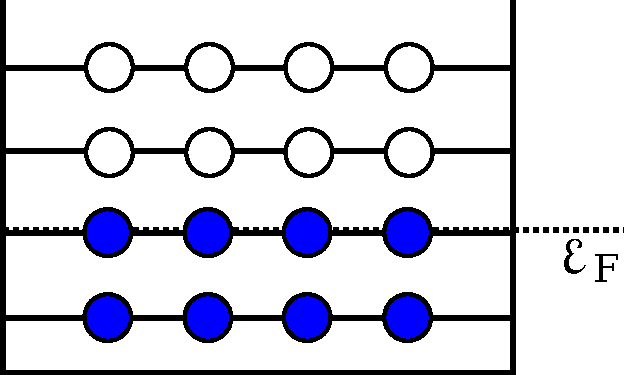
\includegraphics[height=4cm]{manybody/IPM.pdf}}}} 
\end{figure}


\section{Second Quantization}
Even with the simplification of the independent-particle model, the many-body Schodinger equation is an unwieldy and complex system of coupled differential equations.  A useful reformulation of this equation is to promote the single-particle orbits to operators in a step known as \textit{second quantization}.  In this framework, a Slater determinant is represented by a string of occupied orbitals,
\begin{equation}
  \Phi\left(\mathbf{r}_{1},\cdots,\mathbf{r}_{A}\right) \equiv \mathcal{A}\phi_{p_{1}}\phi_{p_{2}}\phi_{p_{3}} \cdots \phi_{p_{N}} \equiv \ket{p_{1}p_{2}p_{3} \cdots p_{N}},
\end{equation}
where $\mathcal{A}$ represents a permutation and normalization operator to correspond with Eq.\ \eqref{eq:slaterdeterminant}.  These second-quantized Slater determinants can be constructed with the use of operators corresponding to specific orbitals.  A \textit{creation} operator, $\co{p}$, places a particle in the $p$ orbital, and an \textit{annihilation} operator, $\ao{p}$, removes a particle from the $p$ orbital,
\begin{equation}
  \co{p}\ket{0} = \ket{p} \hspace{2cm} \ao{p}\ket{p} = \ket{0},
\end{equation}
where $\ket{0}$ represents the vacuum.  Because there must be a correspondance between the original first quantization and second quantization, these creation an annihilation operators obey the following anticommutation ($[ \hat{A},\hat{B} ]_{+} = \hat{A}\hat{B} + \hat{A}\hat{B}$) relations,
\begin{equation} \label{eq:anticommutation}
  [ \co{p},\ao{q} ]_{+} = \delta_{pq} \hspace{1cm} [ \co{p},\co{q} ]_{+} = [ \ao{p},\ao{q} ]_{+} = 0,
\end{equation}
which guarantee that wavefunctions comprised of these operators obey antisymmetry and the Pauli exclusion principle required of fermionic systems.

The Hamiltonian in second-quantized form is,
\begin{equation}
  \Ham = \sum_{\mathclap{pq}}\Hint{1}{p}{q}\ \co{p}\ao{q} + \frac{1}{4}\sum_{\mathclap{pqrs}}\Hint{2}{pq}{rs}\ \co{p}\co{q}\ao{s}\ao{r} + \frac{1}{36}\sum_{\mathclap{pqrstu}}\Hint{3}{pqr}{stu}\ \co{p}\co{q}\co{r}\ao{u}\ao{t}\ao{s} + \cdots,
\end{equation}
where the prefactors account for the double counting of particle-particle interactions and the matrix elements represent integrals over the relavent single-particle wavefunctions,
\begin{gather}
    \Hint{1}{p}{q} \equiv \int d\mathbf{r}_{1}\  \phi^{*}_{p}\left(\mathbf{r}_{1}\right) \HamB{1}\left(\mathbf{r}_{1}\right) \phi_{q}\left(\mathbf{r}_{1}\right) \notag \\
    \Hint{2}{pq}{rs} \equiv \int d\mathbf{r}_{1} d\mathbf{r}_{2}\  \phi^{*}_{p}\left(\mathbf{r}_{1}\right)\phi^{*}_{q}\left(\mathbf{r}_{2}\right) \HamB{2}\left(\mathbf{r}_{1},\mathbf{r}_{2}\right) \phi_{r}\left(\mathbf{r}_{1}\right)\phi_{s}\left(\mathbf{r}_{2}\right) \notag \\
    \Hint{3}{pqr}{stu} \equiv \int d\mathbf{r}_{1} d\mathbf{r}_{2} d\mathbf{r}_{3}\  \phi^{*}_{p}\left(\mathbf{r}_{1}\right)\phi^{*}_{q}\left(\mathbf{r}_{2}\right)\phi^{*}_{r}\left(\mathbf{r}_{3}\right) \HamB{3}\left(\mathbf{r}_{1},\mathbf{r}_{2},\mathbf{r}_{3}\right) \phi_{s}\left(\mathbf{r}_{1}\right)\phi_{t}\left(\mathbf{r}_{2}\right)\phi_{u}\left(\mathbf{r}_{3}\right).
\end{gather}
These definitions apply regardless of the form of the Hamiltonian, and thus this formalism remains generic to the particular system.  This is a crucial step in simplifying the many-body Schrodinger equation because it folds all the complexity of the single-particle wavefunctions and Hamiltonian operators into precomputed matrix elements such that the remaining effort is reduced to algebraic expressions involving creation and annihilation operators.


\section{Normal Ordering}
It's convenient to define a reference state, where states are filled from the true vacuum up to a certin Fermi level.
\begin{equation}
  \refket = \normord{\prod_{i}^{A}\co{i}}\vacket
\end{equation}
This reference determinant defines a Fermi vacuum and states can be defined relative to this vacuum. States above the Fermi vacuum are called \textit{particle} states and will be denoted with the indices $a,b,c,d...$ while states below the Fermi vacuum are called \textit{hole} states and will be denoted with the indeces $i,j,k,l...$. Generic states above or below the Fermi vacuum will be denoted with the indices $p,q,r,s...$.

Any other Slater determinant can be constructed relative to this reference state by adding particles and/or removing holes.  A Slater determinant with $A$ particles added and $B$ holes removed from reference state is known as a $\ph{A}{B}$ excitation.
\begin{align}
  \ket{\Phi^{a}_{i}} &\equiv \co{a}\ao{i}\ket{\Phi} \hspace{2cm} \notag \\
  \ket{\Phi^{ab}_{ij}} &\equiv \co{a}\co{b}\ao{j}\ao{i}\ket{\Phi} \notag \\
  \ket{\Phi^{a}} &\equiv \co{a}\ket{\Phi} \notag \\
  \ket{\Phi_{i}} &\equiv \ao{i}\ket{\Phi}
\end{align}

\begin{figure}
    \centering
  \begin{subfigure}{\textwidth}
    \centering
    \ket{\Phi^{a}_{i}}\ = \vcenter{\hbox{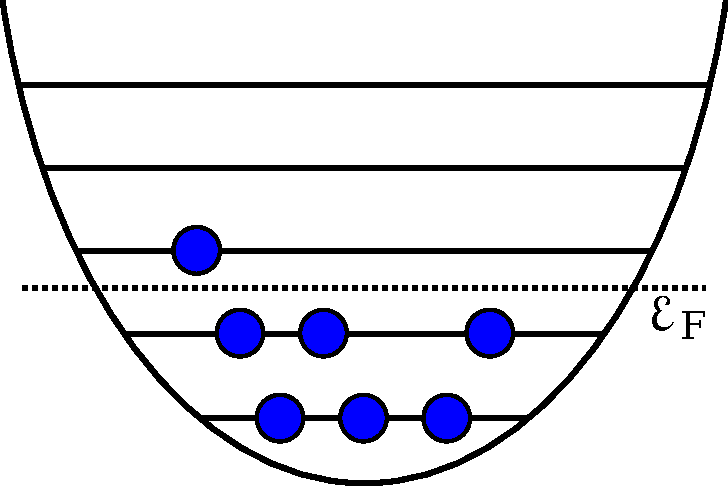
\includegraphics[height=3cm]{manybody/1p1h.pdf}}}} \hspace{2cm} \ket{\Phi^{ab}_{ij}}\ = \vcenter{\hbox{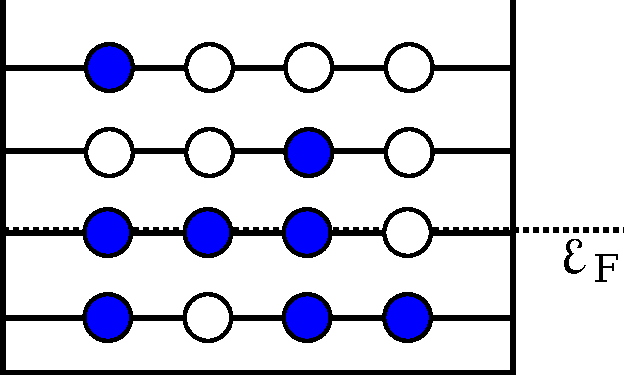
\includegraphics[height=3cm]{manybody/2p2h.pdf}}}}
  \end{subfigure}
  \vspace{0.5cm}
  
  \begin{subfigure}{\textwidth}
    \centering
    \ket{\Phi^{a}}\ = \vcenter{\hbox{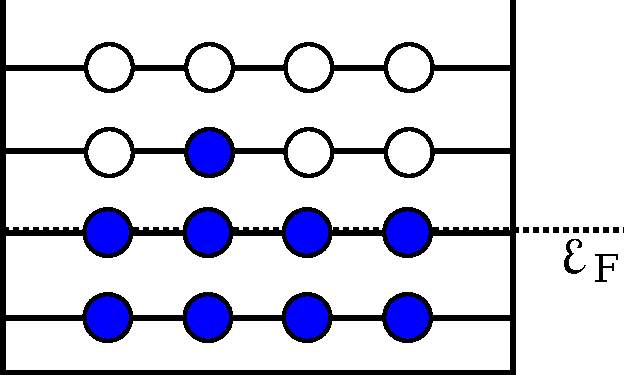
\includegraphics[height=3cm]{manybody/PA.pdf}}}} \hspace{2cm} \ket{\Phi_{i}}\ = \vcenter{\hbox{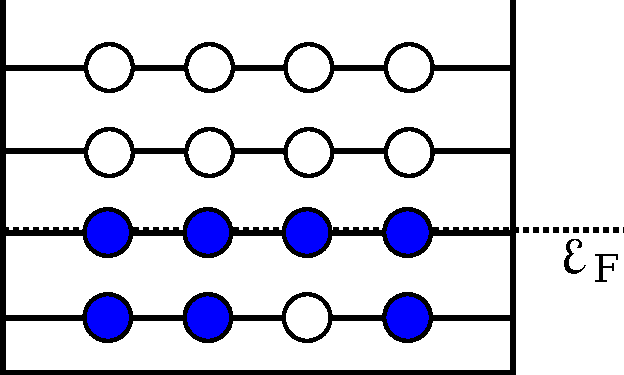
\includegraphics[height=3cm]{manybody/PR.pdf}}}}
  \end{subfigure}
  \caption{Nuclear Chart blah blah blah ab-initio}
  \label{fig:excitations}
\end{figure}
  
Using these definitions, hole-creation and particle-annihilation operators vanish when acting on the Fermi vacuum from the left, $\co{i}\refket=\ao{a}\refket=0$. Conversely, hole-annihilation and particle-creation operators vanish when acting on the Fermi vacuum from the right, $\refbra\ao{i}=\refbra\co{a}=0$.

These results can be exploited to simplify expressions involving strings of creation and annihilation operators by a procedure called \textit{normal ordering} with respect to the Fermi vacuum. Denoted by $\normord{\cdots}$, normal ordering permutes a string of creation and annihilation operators so that hole-annihilation and particle-creation operators are to the left of hole-creation and particle-annihilation operators, which guarantees that normal ordered operators vanish on the Fermi vacuum.
\begin{equation} \label{eq:normorddef}
  \normord{\co{j}\cdots\ao{i}\cdots\ao{b}\cdots\co{a}} = (-1)^{\sigma}\ao{i}\cdots\co{a}\cdots\co{j}\cdots\ao{b},
\end{equation}
where $\sigma$ is the number of two-state permutations required to do the normal ordering.


\section{Wick's Theorem}
At this point, the many-body problem has been reduced to computing long strings of creation and annihilation operators between the normal-ordered Hamiltonian and the correlated wavefunction using Eq.\ \eqref{eq:anticommutation}.  Instead of using a brute-force approach by permuting over and over, a further simplification can be introduced.  A Wick contraction of two operators with respect to the reference state is defined as
\begin{equation} \label{eq:wick1}
  \contraction[1.0ex]{}{\hat{A}}{}{\hat{B}}
  \hat{A}\hat{B} = \hat{A}\hat{B} - \normord{\hat{A}\hat{B}}.
\end{equation}
Which, given the definition in Eq.\ \eqref{eq:normorddef} and the anticommutation relations int Eq.\ \eqref{eq:anticommutation}, means that the only nonzero contractions are of the form,
\begin{equation} \label{eq:wick2}
  \contraction[1.0ex]{}{\hat{a}}{^{\dagger}_{i}}{\hat{a}}
  \hat{a}^{\dagger}_{i}\hat{a}_{j} = \delta_{ij} \hspace{1.0cm} \text{and} \hspace{1.0cm}
  \contraction[1.0ex]{}{\hat{a}}{_{a}}{\hat{a}}
  \hat{a}_{a}\hat{a}_{b}^{\dagger} = \delta_{ab}.
\end{equation}
Because contracted operators simply represent a Kronecker delta, they can be removed from a normal ordered product by permuting the product $\sigma$ times so that the contracted operators are next to each other,
\begin{equation} \label{eq:wick3}
  \contraction[1.0ex]{\{ \hat{A}\cdots}{\hat{B}}{\cdots}{\hat{C}}
  \{ \hat{A}\cdots\hat{B}\cdots\hat{C}\cdots\hat{D} \} = (-1)^{\sigma}
  \contraction[1.0ex]{\{ \hat{A}\cdots}{\hat{B}}{}{\hat{C}}
  \{ \hat{A}\cdots\hat{B}\hat{C}\cdots\hat{D} \} = (-1)^{\sigma}
  \contraction[1.0ex]{}{\hat{B}}{}{\hat{C}}
  \hat{B}\hat{C}\{ \hat{A}\cdots\hat{D} \}.
\end{equation}
These different definitions for operator manipulation come together to define the time-independent Wick's theorem, which reformulates a product of operators as the sum of its normal-ordered form and all possible contractions of its normal-ordered form.
\begin{equation} \label{eq:wick4}
  \hat{A}\hat{B}\hat{C}\cdots\ &=\ \normord{\hat{A}\hat{B}\hat{C}\cdots}\
  +\ \sum_{\mathclap{\substack{\text{one-} \\ \text{contractions}}}}
  \contraction[1.0ex]{\{ }{\hat{A}}{\hat{B}\hat{C}}{\cdots}
  \{ \hat{A}\hat{B}\hat{C}\cdots \}\
   +\ \sum_{\mathclap{\substack{\text{two-} \\ \text{contractions}}}}
   \contraction[0.8ex]{\{ }{\hat{A}}{\hat{B}\hat{C}}{\cdots}
   \contraction[1.2ex]{\{ \hat{A}}{\hat{B}}{\hat{C}\cdots}{}
   \{ \hat{A}\hat{B}\hat{C}\cdots \}\
   +\ \cdots\ +\ \sum_{\mathclap{\substack{\text{all-} \\ \text{contractions}}}}
   \contraction[0.6ex]{\{ }{\hat{A}}{\hat{B}\hat{C}}{\cdots}
   \contraction[1.0ex]{\{ \hat{A}}{\hat{B}}{\hat{C}\cdots}{\ }
   \contraction[1.4ex]{\{ \hat{A}\hat{B}}{\hat{C}}{\cdots\ \ \ }{}
   \{ \hat{A}\hat{B}\hat{C}\cdots\ \ \ \}
\end{equation}

Wick's theorem is incredibly useful in many-body techniques because complicated expressions of operators can be expressed as simple diagrams that are easy to compute with diagrammatic rules which correspond to Eqs.\ \eqref{eq:anticommutation},\eqref{eq:wick2}, and \eqref{eq:wick3}.  These diagrammatic techniques are an integral component to deriving expressions used in this work, and their underlying rules are summarized in \ref{chapter:appendix_diagrams} and are extensively discussed in \cite{SHAVITT2009}.

A powerful application of Wick's theorem is to rewrite the Hamiltonian in normal-ordered form.  This has the effect of shuffling higher-order interactions into lower-order terms, and makes it feasible to include computationally expensive many-body interactions as normal-ordered few-body interactions.  Also, it reorganizes many-body correlations into the reference state so that additional correlations around the Fermi surface can be treated as a perturbation.
\begin{equation}
  \Ham = E_{0} + \sum_{\mathclap{pq}}\fint{p}{q}\normord{\co{p}\ao{q}} + \frac{1}{4}\sum_{\mathclap{pqrs}}\vint{pq}{rs}\normord{\co{p}\co{q}\ao{s}\ao{r}} + \frac{1}{36}\sum_{\mathclap{pqrstu}}\wint{pqr}{stu}\normord{\co{p}\co{q}\co{r}\ao{u}\ao{t}\ao{s}} + \cdots,
\end{equation}
where the newly defined normal-ordered Hamiltonian terms are defined as,
\begin{align}
  E_{0} &= \diagram{Hamiltonian/Hamiltonian-figure0} + \diagram{Hamiltonian/Hamiltonian-figure1} + \diagram{Hamiltonian/Hamiltonian-figure2} + \cdots \notag \\
  &= \sum_{\mathclap{i}}\Hint{1}{i}{i} + \frac{1}{2}\sum_{\mathclap{ij}}\Hint{2}{ij}{ij} + \frac{1}{6}\sum_{\mathclap{ijk}}\Hint{3}{ijk}{ijk} \cdots
\end{align}
\begin{align}
  \diagram{Hamiltonian/Hamiltonian-figure3} &= \diagram{Hamiltonian/Hamiltonian-figure4} + \diagram{Hamiltonian/Hamiltonian-figure5} + \diagram{Hamiltonian/Hamiltonian-figure6} + \cdots \notag \\
  \fint{p}{q} &= \Hint{1}{p}{q} + \sum_{\mathclap{i}}\Hint{2}{pi}{qi} + \frac{1}{2}\sum_{\mathclap{ij}}\Hint{3}{pij}{qij} + \cdots
\end{align}
\begin{align}
  \diagram{Hamiltonian/Hamiltonian-figure7} &= \diagram{Hamiltonian/Hamiltonian-figure8} + \diagram{Hamiltonian/Hamiltonian-figure9} + \cdots \notag \\
  \vint{pq}{rs} &= \Hint{2}{pq}{rs} + \sum_{\mathclap{i}}\Hint{3}{pqi}{rsi} + \cdots
\end{align}
\begin{align}
  \diagram{Hamiltonian/Hamiltonian-figure10} &= \diagram{Hamiltonian/Hamiltonian-figure11} + \cdots \notag \\
  \wint{pqr}{stu} &= \Hint{3}{pqr}{stu} + \cdots
\end{align}

In this form, the Hamiltonian is written is as a sum of the \textit{reference energy}, $E_{0}$, which is the fully-contracted expectation value of the Hamiltonian with respect to the reference state,
\begin{equation}
  E_{0} = \element{\Phi}{\Ham}{\Phi},
\end{equation}
and the remaining normal-ordered pieces of the Hamiltonian, $\HamN$.  Rewriting the many-body Schrodinger equation using this partition gives,
\begin{align}
  &\Ham\ket{\Psi} = (E_{0} + \HamN)\ket{\Psi} = E\ket{\Psi} \notag \\
  \longrightarrow\ \ &\HamN\ket{\Psi} = (E - E_{0})\ket{\Psi} = \Ecorr\ket{\Psi},
\end{align}
where $\Ecorr$ is known as the \textit{correlation energy}.  This shows that further approximations to the Schrodinger equation can be performed with the normal-ordered Hamiltonian and the reference energy.  From this point forward, interactions beyond the three-body level will be ignored.  Electronic systems are naturally truncated at the two-body Coulomb force, while nuclear systems can be succesfully described with the normal-ordered piece of the three-body force and the alternative of keeping higher-ordered interactions is computationally impractical.

Now that the many-body quantum problem has been formulated, different approaches to solving that problem can be proposed and analyzed.  Because taking account of correlations from all particles simultaneously is a demanding--and for some systems, computationally impossible--endeavor, methods for solving the many-body Schrodinger equation should be systematically improvable. Successful methods with this quality incorporate the most dominant correlations in lower-order solutions an approach the exact solution when more and more orders are included.

\section{Hartree--Fock Method}
A successful first-order approximation to any many-body method comes from noticing that each individual particle feels a mean-field potential from the cumulative interactions with all the other particles.  The \textit{Hartree-Fock} (HF) method aims to tranform the original single-particle basis to a Hartree-Fock basis where each orbital is the eigenfunction of its corresponding mean-field.  Because the transformation of a single orbital changes its effect on every other particle, this process must be performed iteratively until self-consistency between all the orbitals is reached, which is why this method is also known as the \textit{Self-Consistent Field} (SCF) method.

This mean-field picture results from the following procedure.  It begins by minimizing the reference energy with respect to the reference state.  This functional is just the zero-body piece of the normal-ordered Hamiltonian,
\begin{equation}
  E_{\text{HF}}\left[ \Phi \right] = \element{\Phi}{\Ham}{\Phi} = \sum_{\mathclap{i}}\Hint{1}{i}{i} + \frac{1}{2}\sum_{\mathclap{ij}}\Hint{2}{ij}{ij} + \frac{1}{6}\sum_{\mathclap{ijk}}\Hint{3}{ijk}{ijk}.
\end{equation}
Transforming the reference determinant can be accomplished by rotating the state within the single-particle basis by use of the \textit{Thouless theorem}, which states that any Slater determinant can be written as the product of any other Slater determinant and an exponentiated single-excitation operator,
\begin{equation} \label{eq:thouless}
  \ket{\Phi'} = e^{\hat{C}_{1}}\ket{\Phi_{0}}, \hspace{1cm} \text{where\ \ } \hat{C}_{1} = \sum_{a i}C^{a}_{i}\normord{ \co{a}\ao{i} }.
\end{equation}
If the difference between the two Slater determinants is dominated by single excitations, this transformation can be approximated by expanding the exponential and ignoring higher-order terms,
\begin{equation} \label{eq:thouless_limit}
  \ket{\Phi'} \simeq \left( 1 + \sum_{a i}C^{a}_{i}\normord{ \co{a}\ao{i} } \right)\ket{\Phi_{0}}.
\end{equation}

The reference energy functional can now be written as a sum of the original reference state and new terms that incorporate the single-excitation variation,
\begin{equation} \label{eq:hf_thouless}
  E_{\text{HF}}\left[ \Phi' \right] = \element{\Phi'}{\Ham}{\Phi'} \simeq E_{\text{HF}}\left[ \Phi \right] + \sum_{a i}C^{a}_{i}\refbra\Ham\ket{\Phi^{a}_{i}} + \sum_{a i}C^{a*}_{\ i}\bra{\Phi^{a}_{i}}\Ham\refket.
\end{equation}
The minimum of this functional is found by varying the coefficients $C^{a}_{i}$ and setting the result to zero,
\begin{equation} \label{eq:del_hf_thouless}
  \delta E_{\text{HF}}\left[ \Phi' \right] \simeq \sum_{a i}\delta C^{a}_{i}\refbra\Ham\ket{\Phi^{a}_{i}} + \sum_{a i}\delta C^{a*}_{\ i}\bra{\Phi^{a}_{i}}\Ham\refket = 0
\end{equation}

Because this expression is Hermitian, both terms must vanish independently so that,
\begin{equation} \label{eq:brillouin}
  \refbra\Ham\ket{\Phi^{a}_{i}} = \bra{\Phi^{a}_{i}}\Ham\refket = 0.
\end{equation}
This condition is the result of the \textit{Brillouin theorem}, which states that the Hamiltonian matrix element must vanish between an optimized Hartree-Fock ground state and any single excitation from it. The Brillouin condition is satisfied by diagonalizing the one-body piece of the normal-ordered Hamiltonian $\fint{p}{q}$, known as the \textit{Fock} operator, such that off-diagonal pieces like $\refbra\Ham\ket{\Phi^{a}_{i}} = \fint{i}{a}$ and $\bra{\Phi^{a}_{i}}\Ham\refket = \fint{a}{i}$ vanish.
\begin{align}
  \diagram{Hamiltonian/Hamiltonian-figure3} &= \diagram{Hamiltonian/Hamiltonian-figure4} + \diagram{Hamiltonian/Hamiltonian-figure5} + \diagram{Hamiltonian/Hamiltonian-figure6} \notag \\
  \fint{p}{q} &= \Hint{1}{p}{q} + \sum_{\mathclap{i}}\Hint{2}{pi}{qi} + \frac{1}{2}\sum_{\mathclap{ij}}\Hint{3}{pij}{qij}\ \ \longrightarrow\ \ \varepsilon^{p}_{q}\delta_{pq},
\end{align}
where $\varepsilon^{p}_{q}$ is the eigenvalue of the Fock operator.

A practical way of solving this system of equations is to express each new orbital in the unknown Hatree-Fock basis, $\ket{p'} \equiv \phi_{p'}\left(\mathbf{r}\right)$, denoted with primed labels, as a linear combination of the known single-particle basis states, $\ket{p} \equiv \phi_{p}\left(\mathbf{r}\right)$, denoted without primed labels.
\begin{equation}
  \ket{p'} = \sum_{p}\braket{p}{p'}\ket{p} = \sum_{p}C^{p}_{p'}\ket{p}
\end{equation}
Then the Fock matrix can be written in terms of the Hartree-Fock basis,
\begin{gather}
  \fint{p'}{q'} = \Hint{1}{p'}{q'} + \sum_{\mathclap{i'}}\Hint{2}{p'i'}{q'i'} + \frac{1}{2}\sum_{\mathclap{i'j'}}\Hint{3}{p'i'j'}{q'i'j'} \notag \\
  = \sum_{\mathclap{pq}}C^{p'*}_{p}\Hint{1}{p}{q}C^{q}_{q'} + \sum_{\mathclap{\substack{i' \\ prqs}}}C^{p'*}_{p}C^{i'*}_{r}\Hint{2}{pr}{qs}C^{q}_{q'}C^{s}_{i'} + \frac{1}{2}\sum_{\mathclap{\substack{i'j' \\ prsqtu}}}C^{p'*}_{p}C^{i'*}_{r}C^{j'*}_{s}\Hint{3}{prs}{qtu}C^{q}_{q'}C^{t}_{i'}C^{u}_{j'}.
\end{gather}
Defining the first-order density matrix $\gamma^{p}_{q}$ as the product of expansion coefficients, summed over all shared hole states,
\begin{equation}
  \gamma^{p}_{q} = \sum_{i'}C^{p}_{i'}C^{i'*}_{q},
\end{equation}
this equation is simplified to,
\begin{equation}
  \fint{p'}{q'} = \sum_{\mathclap{pq}}C^{p'*}_{p}\left[ \Hint{1}{p}{q} + \sum_{\mathclap{rs}}\gamma^{r}_{s}\Hint{2}{pr}{qs} + \frac{1}{2}\sum_{\mathclap{rstu}}\gamma^{r}_{t}\gamma^{s}_{u}\Hint{3}{prs}{qtu} \right]C^{q}_{q'}\ \ \longrightarrow\ \ \varepsilon^{p'}_{q'}\delta_{p'q'}.
\end{equation}
Therefore, the Hartree-Fock equations are ultimately expressed as an eigenvalue problem where the matrix to diagonalize is the Fock matrix in the form,
\begin{equation}
  \hat{F}^{p}_{q}\left(\hat{C}\right) = \Hint{1}{p}{q} + \sum_{\mathclap{rs}}\gamma^{s}_{r}\Hint{2}{pr}{qs} + \frac{1}{2}\sum_{\mathclap{rstu}}\gamma^{t}_{r}\gamma^{u}_{s}\Hint{3}{prs}{qtu},
\end{equation}
and the matrix of coefficients, $\hat{C} = C^{p}_{p'}$, is the unitary operator that transforms the matrix to a diagonal form,
\begin{equation}
  \sum_{\mathclap{pq}}C^{p'*}_{p}F^{p}_{q}\left(\hat{C}\right)C^{q}_{q'} = \varepsilon^{p'}_{q'}\delta_{p'q'}
\end{equation}
The iterative nature of the solution comes from the dependence of the Fock matrix on the transformation coefficients. These Hartree-Fock equations are solved numerically by using an iterative algorithm where the Fock matrix is built using a known set of coefficients and diagonalized to obtain an updated set of coefficients.  This process is repeated until the unitary set of coefficients is unchanged within a certain tolerance.  For most calculations, using the identity matrix as an initial guess for the coefficients is sufficient.  To improve the rate of convergence, techniques such as the direct inversion of the iterative subspace (DIIS) \cite{PULAY1980393,PULAY1982556} or Broyden's method \cite{BROYDEN1965557} can be implemented.  And, to avoid any oscilliatory behavior around the solution, techniques such as the level-shifting method or \textit{ad hoc} linear mixing can be implemented to dampen the large changes between iterations.

To make use of the HF solution as the reference state for post-HF calculations, the Hamiltonian matrix elements must be transformed to the new basis and the normal-ordered version redefined to account for the additional reordering of one-particle correlations into the HF energy.
\begin{gather}
  \fint{p'}{q'} = \varepsilon^{p'}_{q'}\delta_{p'q'} \\
  \vint{p'q'}{r's'} = \sum_{\mathclap{pqrs}} C^{p'*}_{p}C^{q'*}_{q}\left(\Hint{2}{pq}{rs} + \Hint{3}{pqt}{rsu}\gamma^{u}_{t}\right)C^{r}_{r'}C^{s}_{s'} \\
  E_{0} = \sum_{\mathclap{i'}}\Hint{1}{i'}{i'} + \frac{1}{2}\sum_{\mathclap{i'j'}}\Hint{2}{i'j'}{i'j'} + \frac{1}{6}\sum_{\mathclap{i'j'k'}}\Hint{3}{i'j'k'}{i'j'k'} \notag \\
  = \sum_{\mathclap{i'}}\varepsilon^{i'}_{i'} - \frac{1}{2}\sum_{\mathclap{i'j'}}\vint{i'j'}{i'j'} + \frac{1}{6}\sum_{\mathclap{i'j'k'}}\Hint{3}{i'j'k'}{i'j'k'}
\end{gather}
Additionally, any operators that are constructed in the original basis must be transformed in a similar manner.  For example, a one-body operator $\hat{O}$ in the Hartree-Fock basis is,
\begin{gather}
  \hat{O} = \sum_{\mathclap{p'q'}}\opint{}{p'}{q'}\normord{\co{p'}\ao{q'}} = \sum_{\mathclap{p'q'pq}}C^{p'*}_{p}\opint{}{p}{q}C^{q}_{q'}\normord{\co{p'}\ao{q'}} \notag \\
  \longrightarrow\ \ \ \opint{}{p'}{q'} = \sum_{\mathclap{pq}}C^{p'*}_{p}\opint{}{p}{q}C^{q}_{q'}.
\end{gather}

Because the Hartree-Fock basis is diagonal in the one-body piece of the Hamiltonian, any terms that include off-diagonal elements automatically vanish which greatly simplifies any post-Hartree-Fock methods.  From this point, any calculations will use the Hartree-Fock basis unless stated otherwise, and prime symbols will be omitted.  Also, the normal-ordered Hamiltonian will be truncated at the two-body level so that any three-body interactions are included in a cost-effective way.


\section{Configuration-Interaction}
The most generic way to write a correlated wavefunction in a given basis is as a linear combination of all possible Slater determinants.  In normal-ordered form, this expansion can, in principle, consist of the $\ph{0}{0}$ reference state and all possible $\ph{N}{N}$ excitations up to $\ph{A}{A}$ excitations,
\begin{equation} \label{eq:ci_expansion}
  \ket{\Psi_{\nu}} = \sum_{\nu_{i}}^{\mathcal{N}}C_{\nu_{i}}\ket{\Phi_{\nu_{i}}} = C_{0}\ket{\Phi_{0}} + \sum_{N=1}^{A}\left(\frac{1}{N!}\right)^2 \sum_{\substack{a_{1} \ldots a_{N} \\ i_{1} \ldots i_{N}}} C^{a_{1} \ldots a_{N}}_{i_{1} \ldots i_{N}}\ket{\Phi^{a_{1} \ldots a_{N}}_{i_{1} \ldots i_{N}}}.
\end{equation}
Using this form in the many-body Schrodinger equation results in a matrix eigenvalue problem where the matrix elements are Hamiltonian terms that connect two Slater determinants and the eigenvectors are the ground and excited states in the form of Eq.\ \eqref{eq:ci_expansion},
\begin{gather}
  \HamN\ket{\Psi_{\nu}} = \Ecorr_{\nu}\ket{\Psi_{\nu}} \notag \\
  \longrightarrow\ \ \element{\Psi_{\mu}}{\HamN}{\Psi_{\nu}} = \Ecorr_{\nu}\braket{\Psi_{\mu}}{\Psi_{\nu}} \notag \\
  \longrightarrow\ \ \sum_{\mathclap{\mu_{i}\nu_{i}}}C^{*}_{\mu_{i}}\element{\Phi_{\mu_{i}}}{\HamN}{\Phi_{\nu_{i}}}C_{\nu_{i}} = \Ecorr_{\nu}\sum_{\mathclap{\mu_{i}\nu_{i}}}C^{*}_{\mu_{i}}C_{\nu_{i}}\delta_{\mu_{i}\nu_{i}} \notag \\
  \longrightarrow\ \ \mathbf{C}^{\text{T}}_{\mu}\left(\element{\Phi_{\mu_{i}}}{\HamN}{\Phi_{\nu_{i}}} - \Ecorr_{\nu}\mathbf{I}\right)\mathbf{C}_{\nu} = 0.
\end{gather}
The matrix elements can be found with the help of the Slater-Condon rules which, because at this point the Hamiltonian is restricted to one- and two-body terms, require that any Slater determinants which differ by more than two single-particle states vanish.  Also, because the one-body Hamiltonian is diagonal in the Hatree-Fock basis, it only contributes to diagonal elements the CI matrix.  Some examples of these matrix elements are,
\begin{gather}
  \element{\Phi^{a}_{i}}{\Ham}{\Phi^{a}_{i}} = \Edenom{}{a} - \Edenom{}{i} - \vint{ia}{ia} \\
  \element{\Phi^{ab}_{ij}}{\Ham}{\Phi^{cd}_{ij}} = \vint{ab}{cd} \\
  \element{\Phi^{abc}_{ijk}}{\Ham}{\Phi^{abd}_{ijl}} = -\vint{lc}{kd}
\end{gather}

Because the configuration-interaction method exhaustively captures all the correlations of a many-body system, it is considered an ``exact'' method within a certain model space and becomes truely exact as the number of single-particle states is increased to infinity.  However, there is a price to pay for this exactness.  The number of Slater determinants, $\mathcal{N}$, in a model space scales factorially according to Eq.\ \eqref{eq:factorialscaling} and the configuration-interaction matrix scales as $\mathcal{N}^{2}$.  For sufficiently-sized model spaces, the memory required for this matrix quickly becomes unmanigable even for the largest supercomputers.
\begin{figure}
  \centering
  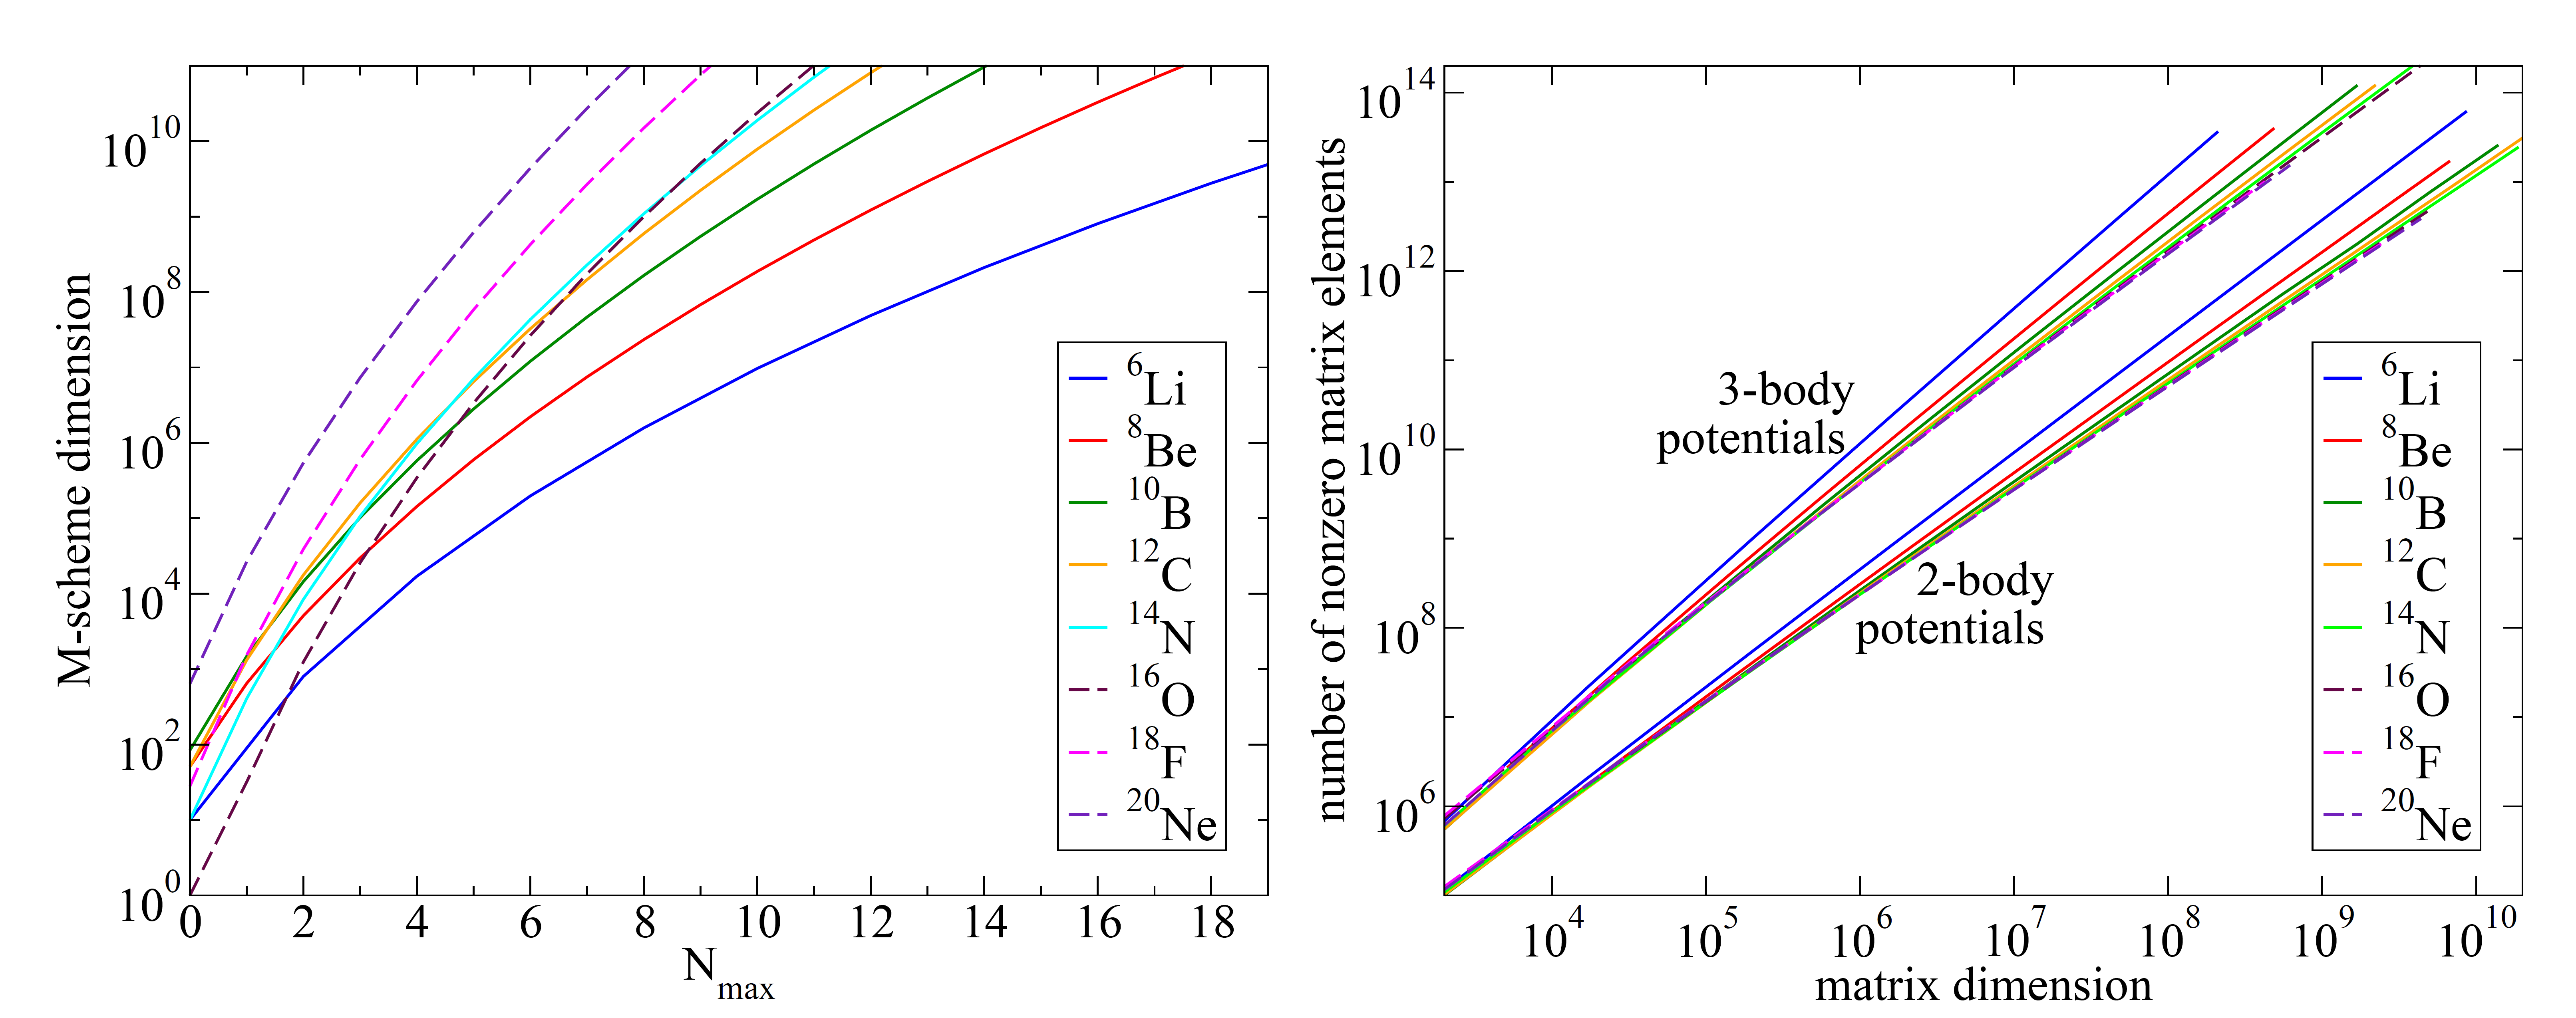
\includegraphics[width=\textwidth]{manybody/FCIscaling.png}
  \caption{Taken from \cite{SHAO2016}}
  \label{fig:fciscaling}
\end{figure}

However, for a reference state that is a good approximation to the true ground state, few-body excitations generally dominate the wavefunctions for low-lying states.  This can be exploited by truncating the expansion in Eq.\ \eqref{eq:ci_expansion}.  Owing to the two-body nature of the interaction, the lowest appropriate truncation is also at the two-body level, known as configuration interaction with singles and doubles (CISD),
\begin{equation} \label{eq:cisd_expansion}
  \ket{\Psi_{\nu}} = C_{0}\ket{\Phi_{0}} + \sum_{\mathclap{a i}} C^{a}_{i}\ket{\Phi^{a}_{i}} + \frac{1}{4}\sum_{\mathclap{a b i j}} C^{ab}_{ij}\ket{\Phi^{ab}_{ij}}.
\end{equation}
This is a very straightforward and tractable way to approximate the many-body Schrodinger equation, and it can be systematically improved by adding more excitations such as triples (CISDT) or triples and quadruples (CISDTQ).  But the drawback to this simplicity is that any truncated CI method is not size-extensive such that any extensive property of a system, like the energy, scales with the size of the system.  A desirable many-body method will be both systematically improvable and size-extensive while maintaining computational feasibility.

\section{Many-Body Perturbation Theory}

\begin{gather}
  \Ham = \Ham_{0} + \lambda\hat{V},\ \ \text{with} \notag \\
  \Ham_{0} = E_{0} + \sum_{\mathclap{p}}\fint{p}{p}\normord{\co{p}\ao{p}}\ \ \text{and} \notag \\
  \hat{V} = \frac{1}{4}\sum_{\mathclap{pqrs}}\vint{pq}{rs}\normord{\co{p}\co{q}\ao{s}\ao{r}}
\end{gather}
When not in the Hartree-Fock basis, the interaction piece has the additional term, $\sum_{p\neq q}\fint{p}{q}\normord{\co{p}\ao{q}}$.

The reference state is an eigenstate of the zero-order piece of the Hamiltonian,
\begin{equation}
  \Ham_{0}\ket{\Phi} = \left(E_{0} + \sum_{\mathclap{i}}\fint{i}{i}\normord{\co{i}\ao{i}}\right)\ket{\Phi} = \left(E_{0} + \sum_{\mathclap{i}}\Edenom{}{i}\right)\ket{\Phi} = E^{(0)}_{0}\ket{\Phi}
\end{equation}

\begin{gather}
  \Ham\corrket = \mathop{(\Ham_{0} + \hat{V})}\corrket = E\corrket \\
  \refbra\mathop{(\Ham_{0} + \hat{V})}\corrket = \refbra\Ham_{0}\corrket + \refbra\hat{V}\corrket = E\braket{\Phi}{\Psi} \\
  E^{(0)}\braket{\Phi}{\Psi} + \refbra\hat{V}\corrket = E^{(0)} + \refbra\hat{V}\corrket = E \\
  \Delta E_{0} \equiv E - E^{(0)} = \refbra\hat{V}\corrket \label{eq:MBPT_delE}
\end{gather}

\begin{gather}
  \mathop{(\Ham - E)}\ket{\Psi} = 0 \\
  E \equiv E^{(0)} + \Delta E_{0} = E^{(0)} + \lambda E^{(1)} + \lambda^{2} E^{(2)} + \cdots \\
  \ket{\Psi} \equiv \ket{\Phi} + \ket{\mathcal{X}} = \ket{\mathcal{X}^{(0)}} + \lambda\ket{\mathcal{X}^{(1)}} + \lambda^{2}\ket{\mathcal{X}^{(2)}} + \cdots \\
  \mathop{(\Ham_{0} + \lambda\hat{V} - E^{(0)} - \lambda E^{(1)} - \lambda^{2} E^{(2)} - \cdots)}\mathop{(\ket{\mathcal{X}^{(0)}} + \lambda\ket{\mathcal{X}^{(1)}} + \lambda^{2}\ket{\mathcal{X}^{(2)}} + \cdots)} = 0
\end{gather}


Next, the projection operators $\hat{P}$ and $\hat{Q}$ can be introduced,
\begin{gather}
  \hat{P} = \ket{\Phi_{0}}\bra{\Phi_{0}}, \\
  \hat{Q} = \sum_{n\neq 0}\ket{\Phi_{n}}\bra{\Phi_{n}} = 1 - \ket{\Phi_{0}}\bra{\Phi_{0}}.
\end{gather}
The $\hat{P}$ operator isolates the reference-state component of any Slater determinant while the $\hat{Q}$ operator isolates all components \textit{except} the reference-state component out of any Slater determinant.  Both these operators are indempotent, which means that $\hat{P}^{2} = \hat{P}$ and $\hat{Q}^{2} = \hat{Q}$, and because of intermediate normalization, the correlated wavefunction can be written as $\ket{\Psi} = \mathop{(\hat{P} + \hat{Q})}\ket{\Psi} = \ket{\Phi} + \hat{Q}\ket{\Psi}$.  Also, both operators commute with the unperturbed part of the Hamiltonian, $\Ham_{0}\hat{P} = \hat{P}\Ham_{0}$ and $\Ham_{0}\hat{Q} = \hat{Q}\Ham_{0}$.  These identities can be applied to an alternate version of the Schrodinger equation which defines a particular version of pertrubation theory known as Raleigh-Schrodinger perturbation theory (RSPT). In this version, the zeroth-order energy $E^{(0)}$ is added to both sides of the Schrodinger equation.  Acting with $\hat{Q}$ and rearranging terms gives,
\begin{gather}
  \hat{Q}\mathop{(E^{(0)} - \Ham_{0})}\ket{\Psi} = \hat{Q}\mathop{(E^{(0)} + \hat{V} - E)}\ket{\Psi} \notag \\
  \hat{Q}\mathop{(E^{(0)} - \Ham_{0})}\hat{Q}\ket{\Psi} = \hat{Q}\mathop{(\hat{V} - \Delta E_{0})}\ket{\Psi}
\end{gather}
The operator $\hat{Q}\mathop{(E^{(0)} - \Ham_{0})}\hat{Q}$ is invertible because $\mathop{(E^{(0)} - \Ham_{0})^{-1}}$ is never singular in $Q$-space.  Therefore, the operator $\hat{R}_{0} = \hat{Q}\mathop{(E^{(0)} - \Ham_{0})^{-1}}\hat{Q}$, known as the \textit{resolvant}, can be applied to both sides to result in the generating equation for RSPT,
\begin{gather}
  \hat{Q}\mathop{(E^{(0)} - \Ham_{0})^{-1}}\mathop{(E^{(0)} - \Ham_{0})}\hat{Q}\ket{\Psi} = \hat{Q}\mathop{(E^{(0)} - \Ham_{0})^{-1}}\hat{Q}\mathop{(\hat{V} - \Delta E_{0})}\ket{\Psi} \notag \\
  \hat{Q}\ket{\Psi} = \hat{R}_{0}\mathop{(\hat{V} - \Delta E_{0})}\ket{\Psi} \notag \\
  \ket{\Psi} = \ket{\Phi} + \hat{R}_{0}\mathop{(\hat{V} - \Delta E_{0})}\ket{\Psi}
\end{gather}

This equation can be iterated infinitely to give the solution for the fully correlated wave function which can, in turn, be used to solve for the energy with Eq.\ \eqref{eq:MBPT_delE},
\begin{gather}
  \ket{\Psi} = \sum_{n=0}^{\infty}\left[\hat{R}_{0}\mathop{(\hat{V} - \Delta E_{0})}\right]^{n}\ket{\Phi_{0}}, \\
  \Delta E_{0} = \refbra\hat{V}\corrket = \sum_{n=0}^{\infty}\refbra\hat{V}\left[\hat{R}_{0}\mathop{(\hat{V} - \Delta E_{0})}\right]^{n}}\ket{\Phi_{0}}
\end{gather}
The immediate problem with this equation is that the right-hand side of the equations contain the target energy difference \Delta E_{0} for which this equation is meant to solve.


\begin{gather}
  \mathop{(E^{(0)} - H_{0})}\hat{Q}\ket{\Psi} = \hat{Q}\mathop{(E^{(0)} - H_{0})}\ket{\Psi} = Q\mathop{(E^{(0)} - \Ham + \hat{V})}\ket{\Psi} = Q\mathop{(E^{(0)} - E + \hat{V})}\ket{\Psi}
\end{gather}


Assuming that the eigenvalues, $\mathop{E^{(0)}_{n}}$, are non-degenerate, the operator $\mathop{(E^{(0)}_{0}-H_{0})}$ is singular on $\ket{\Phi_{0}}$ but non-singular on the Q-space. Therefore, it can be inverted in the preceding equation,
\begin{equation}
Q\ket{\Psi_{0}}=\mathop{(E^{(0)}_{0}-H_{0})^{-1}}Q\mathop{(E^{(0)}_{0}-H+H_{1})}\ket{\Psi_{0}}=R^{(0)}\mathop{(E^{(0)}_{0}-E_{0}+H_{1})}\ket{\Psi_{0}},
\end{equation}
where $R^{(0)}=\mathop{(E^{(0)}_{0}-H_{0})^{-1}}Q$ is the reduced resolvent of the unperturbed operator $H_{0}$. Expanding an arbitrary term of the resolvant as an infinite series and applying the unperturbed operator gives
\begin{equation}
\mathop{(E^{(0)}_{0}-H_{0})^{-1}}\ket{\Phi_{n}}\bra{\Phi_{n}}=\mathop{(E^{(0)}_{0})^{-1}}\mathop{\left(1-\frac{H_{0}}{E^{(0)}_{0}}\right)^{-1}}\hspace{-4mm}\ket{\Phi_{n}}\bra{\Phi_{n}}=\mathop{(E^{(0)}_{0})^{-1}}\sum_{n=0}^{\infty}\mathop{\left(\frac{H_{0}}{E^{(0)}_{0}}\right)^{n}}\hspace{-2mm}\ket{\Phi_{n}}\bra{\Phi_{n}}
\end{equation}
\begin{equation}
=\mathop{(E^{(0)}_{0})^{-1}}\sum_{n=0}^{\infty}\mathop{\left(\frac{E^{(0)}_{n}}{E^{(0)}_{0}}\right)^{n}}\hspace{-2mm}\ket{\Phi_{n}}\bra{\Phi_{n}}=\mathop{(E^{(0)}_{0})^{-1}}\mathop{\left(1-\frac{E^{(0)}_{n}}{E^{(0)}_{0}}\right)^{-1}}\hspace{-4mm}\ket{\Phi_{n}}\bra{\Phi_{n}}=\mathop{(E^{(0)}_{0}-E^{(0)}_{n})^{-1}}\ket{\Phi_{n}}\bra{\Phi_{n}}.
\end{equation}
From Eqn. (45), the definition of $Q$, and intermediate normalization ($\braket{\Phi_{0}}{\Psi_{0}}=1$),
\begin{equation}
Q\ket{\Psi_{0}}=\ket{\Psi_{0}}-\ket{\Phi_{0}}\braket{\Phi_{0}}{\Psi_{0}}=\ket{\Psi_{0}}-\ket{\Phi_{0}}=R^{(0)}\mathop{(E^{(0)}_{0}-E_{0}+H_{1})}\ket{\Psi_{0}}.
\end{equation}
Now we can define $W=\mathop{(E^{(0)}_{0}-E_{0}+H_{1})}$, drop the superscript from the reduced resolvent, and rearrange the previous equation to give,
\begin{equation}
\ket{\Psi_{0}}=\ket{\Phi_{0}}+RW\ket{\Psi_{0}}
\end{equation}
This equation can be iterated resulting in
\begin{equation}
\ket{\Psi_{0}}=\sum_{n=0}^{\infty}\mathop{(RW)^{n}}\ket{\Phi_{0}}
\end{equation}
The energy is obtained by applying the full Hamiltonian to this expression and multiplying by the unperturbed reference function to the left before applying the intermediate normalization,
\begin{equation}
\bra{\Phi_{0}}\mathop{(H_{0}+H_{1})}\ket{\Psi_{0}}=\bra{\Phi_{0}}\mathop{H_{0}\ket{\Psi_{0}}+\bra{\Phi_{0}}H_{1}}\ket{\Psi_{0}}=\bra{\Phi_{0}}E^{(0)}_{0}\ket{\Psi_{0}}+\bra{\Phi_{0}}H_{1}\ket{\Psi_{0}}
\end{equation}
\begin{equation}
E_{0}=E^{(0)}_{0}\braket{\Phi_{0}}{\Psi_{0}}+\bra{\Phi_{0}}H_{1}\ket{\Psi_{0}}=E^{(0)}_{0}+\element{\Phi_{0}}{\sum_{n=0}^{\infty}\mathop{H_{1}(RW)^{n}}}{\Phi_{0}}
\end{equation}

\begin{gather}
  \diagram{MBPT/MBPT-figure21}\hspace{-0.2cm} + \hspace{-0.2cm}\diagram{MBPT/MBPT-figure22}\hspace{-0.2cm} = \hspace{-0.4cm}\diagram{MBPT/MBPT-figure23} \notag \\
  \frac{1}{16}\sum_{\mathclap{\substack{abcd \\ ijkl}}}\frac{\vint{ij}{ab}\vint{ab}{ij}\vint{kl}{cd}\vint{cd}{kl}}{\Edenom{ab}{ij}\Edenom{abcd}{ijkl}\Edenom{cd}{kl}} + \frac{1}{16}\sum_{\mathclap{\substack{abcd \\ ijkl}}}\frac{\vint{ij}{ab}\vint{ab}{ij}\vint{kl}{cd}\vint{cd}{kl}}{\Edenom{ab}{ij}\Edenom{abcd}{ijkl}\Edenom{ab}{ij}} = \frac{1}{16}\sum_{\mathclap{\substack{abcd \\ ijkl}}}\vint{ij}{ab}\vint{ab}{ij}\vint{kl}{cd}\vint{cd}{kl}\left(\frac{\Edenom{ab}{ij} + \Edenom{cd}{kl}}{\left(\Edenom{ab}{ij}\right)^{2}\Edenom{abcd}{ijkl}\Edenom{cd}{kl}}\right) \notag \\
  = \left(\frac{1}{4}\sum_{\mathclap{abij}}\frac{\vint{ij}{ab}\vint{ab}{ij}}{\left(\Edenom{ab}{ij}\right)^{2}}\right)\left(\frac{1}{4}\sum_{\mathclap{cdkl}}\frac{\vint{kl}{cd}\vint{cd}{kl}}{\Edenom{cd}{kl}}\right) = \braket{\Psi^{(1)}_{n}}{\Psi^{(1)}_{n}}E^{(2)}_{n} = \element{\Phi}{\Vop\Res\Vt\Res\Vt\Res\Vop}{\Phi}_{\text{D}}
\end{gather}

\begin{gather}
  \diagram{MBPT/MBPT-figure24}\hspace{-0.2cm} + \hspace{-0.2cm}\diagram{MBPT/MBPT-figure25}\hspace{-0.2cm} = \hspace{-0.4cm}\diagram{MBPT/MBPT-figure26} \notag \\
  \frac{1}{16}\sum_{\mathclap{\substack{abcd \\ ijkl}}}\frac{\vint{ab}{ij}\vint{kl}{cd}\vint{cd}{kl}}{\Edenom{cd}{kl}\Edenom{abcd}{ijkl}\Edenom{ab}{ij}}\ket{\Phi^{ab}_{ij}} + \frac{1}{16}\sum_{\mathclap{\substack{abcd \\ ijkl}}}\frac{\vint{ab}{ij}\vint{kl}{cd}\vint{cd}{kl}}{\Edenom{ab}{ij}\Edenom{abcd}{ijkl}\Edenom{ab}{ij}}\ket{\Phi^{ab}_{ij}} = \frac{1}{16}\sum_{\mathclap{\substack{abcd \\ ijkl}}}\vint{ab}{ij}\vint{kl}{cd}\vint{cd}{kl}\left(\frac{\Edenom{ab}{ij} + \Edenom{cd}{kl}}{\left(\Edenom{ab}{ij}\right)^{2}\Edenom{abcd}{ijkl}\Edenom{cd}{kl}}\right)\ket{\Phi^{ab}_{ij}} \notag \\
  = \left(\frac{1}{4}\sum_{\mathclap{abij}}\frac{\vint{ab}{ij}}{\left(\Edenom{ab}{ij}\right)^{2}}\ket{\Phi^{ab}_{ij}}\right)\left(\frac{1}{4}\sum_{\mathclap{cdkl}}\frac{\vint{kl}{cd}\vint{cd}{kl}}{\Edenom{cd}{kl}}\right) = \frac{\ket{\Psi^{(1)}_{n}}}{\Edenom{}{n}}E^{(2)}_{n} = \Res\Vt\Res\Vt\Res\Vop\ket{\Phi}_{\text{D}}
\end{gather}




\begin{gather}
  \mathop{(\Ham_{0} - E^{(0)}\cdots)}\mathcal{X}^{(0)} = 0 \\
  \mathop{(\Ham_{0} - E^{(0)})}\mathcal{X}^{(1)} + \mathop{(\hat{V} - E^{(1)})}\mathcal{X}^{(0)} = 0 \\
  \mathop{(\Ham_{0} - E^{(0)})}\mathcal{X}^{(2)} + \mathop{(\hat{V} - E^{(1)})}\mathcal{X}^{(1)} - E^{(2)}\mathcal{X}^{(0)} = 0 \\
  \mathop{(\Ham_{0} - E^{(0)})}\mathcal{X}^{(n)} + \mathop{(\hat{V} - E^{(1)})}\mathcal{X}^{(n-1)} - \sum^{n-2}_{\mathclap{m=0}} E^{(n-m)}\mathcal{X}^{(m)} = 0
\end{gather}

\begin{gather}
  \refbra\mathop{(\Ham_{0} - E^{(0)})}\ket{\mathcal{X}^{(n)}} = \refbra\mathop{(E^{(1)} - \hat{V})}\ket{\mathcal{X}^{(n-1)}} + \refbra\sum^{n-2}_{\mathclap{m=0}} E^{(n-m)}\ket{\mathcal{X}^{(m)}} \\
  \refbra\Ham_{0}\ket{\mathcal{X}^{(n)}} - \refbra E^{(0)}\ket{\mathcal{X}^{(n)}} = \refbra E^{(1)}\ket{\mathcal{X}^{(n-1)}} - \refbra\hat{V}\ket{\mathcal{X}^{(n-1)}} + \sum^{n-2}_{\mathclap{m=0}}\refbra E^{(n-m)}\ket{\mathcal{X}^{(m)}} \\
  \refbra\Ham_{0}\ket{\mathcal{X}^{(n)}} - \refbra E^{(0)}\ket{\mathcal{X}^{(n)}} = - \refbra\hat{V}\ket{\mathcal{X}^{(n-1)}} + \sum^{n-1}_{\mathclap{m=0}}\refbra E^{(n-m)}\ket{\mathcal{X}^{(m)}} \\
  \mathop{(E^{(0)} - E^{(0)})}\braket{\Phi}{\mathcal{X}^{(n)}} = - \refbra\hat{V}\ket{\mathcal{X}^{(n-1)}} + \sum^{n-1}_{\mathclap{m=0}}E^{(n-m)}\braket{\Phi}{\mathcal{X}^{(m)}} \\
  0 = - \refbra\hat{V}\ket{\mathcal{X}^{(n-1)}} + \sum^{n-1}_{\mathclap{m=0}}E^{(n-m)}\delta_{m0} \\
  E^{(n)} = \refbra\hat{V}\ket{\mathcal{X}^{(n-1)}}
\end{gather}

\begin{gather}
  E^{(1)} = \refbra\hat{V}\refket \\
  E^{(n)} = \refbra\hat{V}\ket{\mathcal{X}^{(n-1)}}
\end{gather}



\section{Many-Body Perturbation Theory}
Many-body perturbation theory treats the interaction part of the Hamiltonian, $H_{1}$, as a perturbation using the parameter $\lambda$ to keep track of the perturbation order. The unperturbed Hamiltonian is given when $\lambda=0$ and the full Hamiltonian is restored when $\lambda=1$,
\begin{equation}
H=H_{0}+\lambda H_{1}.
\end{equation}
The solution wave functions to the unperturbed Hamiltonian are given by $\Phi_{n}$ and those for the perturbed Hamiltonian are given by $\Psi_{n}$,
\begin{equation}
H_{0}\ket{\Phi_{n}}=E^{(0)}_{n}\ket{\Phi_{n}}
\end{equation}
\begin{equation}
\mathop{(H_{0}+H_{1})}\ket{\Psi_{n}}=E_{n}\ket{\Psi_{n}}
\end{equation}
If one assumes that the $\Phi_{n}$ are non-degenerate, then the perturbed wave functions and energies become the corresponding non-perturbed wave function and energies when $\lambda\rightarrow 0$. Defining the differences between the full and unperturbed wave functions and energies as $\chi_{n}=\Psi_{n}-\Phi_{n}$ and $\Delta E_{n}=E_{n}-E^{(0)}_{n}$, respectively, I can rewrite the Schrodinger equation as
\begin{equation}
H\mathop{(\Phi_{n}+\chi_{n})}=E_{n}\mathop{(\Phi_{n}+\chi_{n})}
\end{equation}
\begin{equation}
\mathop{(H-E_{n})}\chi_{n}=\mathop{(E_{n}-H)}\Phi_{n}=\mathop{(E_{n}-H_{0}-H_{1})}\Phi_{n}
\end{equation}
\begin{equation}
\mathop{(H-E_{n})}\chi_{n}=\mathop{(E_{n}-E^{(0)}_{n}-H_{1})}\Phi_{n}=\mathop{(\Delta E_{n}-H_{1})}\Phi_{n}
\end{equation}
Because any solution to the homogeneous version of Eqn. (28), $\mathop{(H-E_{n})}\chi_{n}=0$, can be added to the solution of the inhomogeneous version, there exists a degree of freedom that can be used to set $\chi_{n}$ orthogonal to $\Phi_{n}$, $\braket{\chi_{n}}{\Phi_{n}}=0$. This form is known as intermediate normalization and sets the following inner products,
\begin{equation}
\braket{\Phi_{n}}{\Psi_{n}}=\braket{\Phi_{n}}{\Phi_{n}+\chi_{n}}=\braket{\Phi_{n}}{\Phi_{n}}+\braket{\Phi_{n}}{\chi_{n}}=1+0=1,
\end{equation}
\begin{equation}
\braket{\Psi_{n}}{\Psi_{n}}=\braket{\Phi_{n}+\chi_{n}}{\Phi_{n}+\chi_{n}}=\braket{\Phi_{n}}{\Phi_{n}}+\braket{\chi_{n}}{\chi_{n}}=1+\braket{\chi_{n}}{\chi_{n}}.
\end{equation}
Now the perturbation expasion equations can be written by first expanding $\chi_{n}$ and $\Delta E_{n}$ in different orders of $\lambda$ where the zero-order contributions correspond to the unperturbed wave function and energy, respectively.
\begin{equation}
\Psi_{n}=\Phi_{n}+\chi_{n}=\Psi^{(0)}_{n}+\lambda\Psi^{(1)}_{n}+\lambda^{2}\Psi^{(1)}_{n}+...
\end{equation}
\begin{equation}
E_{n}=E^{(0)}_{n}+\Delta E_{n}=E^{(0)}_{n}+\lambda E^{(1)}_{n}+\lambda^{2}E^{(2)}_{n}+...
\end{equation}
Plugging these expansions into the perturbed Hamiltonian, $\mathop{(H_{0}+\lambda H_{1}-E_{n})}\Psi_{n}=0$, gives
\begin{equation}
\mathop{(H_{0}+\lambda H_{1}-E^{(0)}_{n}-\lambda E^{(1)}_{n}-\lambda^{2}E^{(2)}_{n}-...)}\mathop{(\Psi^{(0)}_{n}+\lambda\Psi^{(1)}_{n}+\lambda^{2}\Psi^{(1)}_{n}+...)}=0
\end{equation}
After expanding the expressions in Eqn. (33), different orders of $\lambda$ can be equated to give order-by-order equations for the $\Psi^{(m)}_{n}$ in terms of the lower-order wave functions. In general, the equations are given by
\begin{equation}
\mathop{(E^{(0)}_{n}-H_{0})}\Psi^{(0)}_{n}=0,
\end{equation}
\begin{equation}
\mathop{(E^{(0)}_{n}-H_{0})}\Psi^{(m)}_{n}=H_{1}\Psi^{(m-1)}_{n}-\sum_{l=0}^{m-1}E^{(m-l)}_{n}\Psi^{(l)}_{n}.
\end{equation}
The corresponding order-by-order energies are solved by multiplying Eqn. (35) by $\bra{\Phi_{n}}$ and integrating,
\begin{equation}
\element{\Phi_{n}}{\mathop{(E^{(0)}_{n}-H_{0})}}{\Psi^{(m)}_{n}}=\element{\Phi_{n}}{H_{1}}{\Psi^{(m-1)}_{n}}-\sum_{l=0}^{m-1}E^{(m-l)}_{n}\braket{\Phi_{n}}{\Psi^{(l)}_{n}}.
\end{equation}
The first term is zero because it gives the solution to the unperturbed Hamiltonian, and the inner product in the last term is only non-zero when $l=0$,
\begin{equation}
E^{(m)}_{n}=\element{\Phi_{n}}{H_{1}}{\Psi^{(m-1)}_{n}}.
\end{equation}
We see here that the $n^{\text{th}}$ order wavefunction contains the perturbation to the $\mathop{n-1}^{\text{th}}$ order.




\section{Center-of-Mass Factorization}

\begin{equation}
  \corrket = \corrket_{\text{cm}}\corrket_{\text{in}}
\end{equation}

\begin{equation}
  \Ham_{\text{in}} = \Top - \Top_{\text{cm}} + \Vop = \sum_{i<j}^{A} \left[ \frac{\left( \hat{\mathbf{p}}_{i} - \hat{\mathbf{p}}_{j} \right)^{2}}{2mA} + \Vop\left( \mathbf{r}_{i} - \mathbf{r}_{j} \right) \right]
\end{equation}

By defining the center-of-mass momentum as $\vec{P}=\sum_{i=1}^{A}\vec{p}_{i}$, this separation of the kinetic term gives,
Next, defining the center-of-mass coordinate as $\vec{R}=\frac{1}{A}\sum_{i=1}^{A}\vec{r}_{i}$ allows for the separation of the potential term,

\begin{equation}
  \Ham_{cm}\left( \tilde{\omega} \right) = \Top_{\text{cm}} + \frac{1}{2}mA\tilde{\omega}^{2}\Rop_{\text{cm}}^{2} - \frac{3}{2}\hbar\tilde{\omega} = \frac{1}{2mA}\sum_{ij}^{A}\mathbf{p}}_{i}\cdot\mathbf{p}}_{j} + \frac{m\tilde{\omega}^{2}}{2A}\sum_{ij}^{A}\mathbf{r}_{i}\cdot\mathbf{r}_{j} - \frac{3}{2}\hbar\tilde{\omega}
\end{equation}
  
Use of Jacobi coordinates \cite{BISHOP19901341,NOGGA2002054003}

\begin{equation}
  E_{\text{cm}}\left( \omega \right) \equiv \left\langle \Ham_{cm}\left( \tilde{\omega} \right) \right\rangle \simeq \frac{1}{2\lambda}\left( \left\langle \Ham_{\text{in}} + \lambda\Ham_{cm}\left( \tilde{\omega} \right) \right\rangle - \left\langle \Ham_{\text{in}} - \lambda\Ham_{cm}\left( \tilde{\omega} \right) \right\rangle \right)
\end{equation}

\cite{HAGEN2009062503}
require that $E_{\text{cm}}\left( \tilde{\omega} \right) = 0$ and use $\left\langle \Top_{\text{cm}} \right\rangle = \frac{3}{4}\hbar\tilde{\omega}$
\begin{gather}
  \Ham_{cm}\left( \omega \right) + \frac{3}{2}\hbar\omega - \Top_{\text{cm}} = \frac{\omega^{2}}{\tilde{\omega}^{2}}\left( \Ham_{cm}\left( \tilde{\omega} \right)  + \frac{3}{2}\hbar\tilde{\omega} - \Top_{\text{cm}} \right) \notag \\
  \hbar\tilde{\omega} = \hbar\omega + \frac{2}{3}E_{\text{cm}}\left( \omega \right) \pm \sqrt{\frac{4}{9}\left( E_{\text{cm}}\left( \omega \right) \right)^{2} + \frac{4}{3}\hbar\omegaE_{\text{cm}}\left( \omega \right)}
\end{gather}

Lawson-Gloeckner method, \cite{GLOECKNER1974313}.
\begin{equation} \label{eq:lawsongloeckner}
  \Ham^{\hspace{1pt}}_{\text{in}} = \Ham_{\text{in}} + \beta\Ham_{\text{cm}}\left( \tilde{\omega} \right)
\end{equation}

\end{document}
